\subsection{Experiments}

\subsubsection{Analyzing sensitivity towards the initial estimate}
For this experiment, we use a synthetic signal generated randomly with $n=1000$ and $s=20$. 
Our aim is to analyze the sensitivity of our algorithm towards the initial estimate $\mathbf{x^0}$. %Currently, in the absence of a suitable initialization method, 
For that, we compute the initial estimate $\mathbf{x^0}$ by adding a Gaussian noise to the original signal. In Fig.~\ref{fig:pl}, we plot the variation of the relative reconstruction error ($\frac{\norm{\mathbf{x^*-x^N}}}{\norm{\mathbf{x^*}}}$) with the relative error in initial estimate ($\frac{\norm{\mathbf{x^*-x^0}}}{\norm{\mathbf{x^*}}}$). We plot the similar curves for different values of number of measurements $m$.
\begin{figure}[t]
	\begin{center}
		%\vspace{-0em}
		\includegraphics[width=\linewidth]{./fig/graph.pdf}
	\end{center}
	\caption{}
	\label{fig:pl}
\end{figure}

%\newpage
%\begin{section}{Appendix}
%\begin{figure}[t]
%	\begin{center}
%		\includegraphics[width=0.4\linewidth]{./fig/alg.png}
%	\end{center}
%	\caption{\emph{Our approach}}
%	\label{fig:alg}
%\end{figure}
%\end{section}

\subsubsection{Performance of our algorithm for signal reconstruction}
We perform experiments on a synthetic signal generated randomly with $n=1000$ and $s=5$. We compute the initial estimate $\mathbf{x^0}$ using first order estimator method described in~\ref{sec:init}. we plot the variation of the relative reconstruction error ($\frac{\norm{\mathbf{x^*-x^N}}}{\norm{\mathbf{x^*}}}$) with number of measurements $m$ for both the variants of sparse recovery algorithm as described in~\ref{sec:altmin}.

It is important to note that unlike the absolute value function, the modulo function described in Fig.~\ref{fig:graph} is not scale-invariant. The modulo function works over the quantities $y_{c,i}=\langle \mathbf{a_i} \cdot \mathbf{x^*} \rangle, i=1,..,m$; and it is defined over the parameter $R$; thus depending on the magnitudes of $y_{c,i}$ and $R$ relative to each other, the behavior of the measurement model and the reconstruction algorithm would be altered. For instance, if the value of $R$ is too small compared to the range of the $y_{c,i}$, the modulo operation would hardly have any effect on the measurements, leaving $\mathbf{y_c \approx y}$. To analyze such variations, we fix the $R =1$ in our experiments, while varying the signal strength to vary the magnitudes of $y_{c,i}$. We measure the signal strength by the norm of the original signal ($\norm{\mathbf{{x}^*}}=1$).

Another important factor affecting the reconstruction is the quality of the initial estimate ($\mathbf{{x}^0}$) obtained through first order estimation. As described in~\ref{sec:init}, the quality of the initial estimate is a direct function of number of measurements ($m$). As we set $m$ higher, the initial estimate $\mathbf{{x}^0}$ would move closer to the original signal $\mathbf{{x}^*}$. For our experiments, we consider two ranges of $m$: $m \in [100,1000]$ and $m \in [1000,10000]$.
\begin{center}
	\begin{table}
		\centering
		\begin{tabular}{cccc}\toprule
			\multicolumn{4}{c}{\small{\textbf{Fixed:} $R=1, n=1000, s=5$}} \\ \midrule
			\multicolumn{2}{c}{\textbf{CoSaMP}}&\multicolumn{2}{c}{\textbf{robust CoSaMP}}
			\\\cmidrule(r){1-2}\cmidrule(r){3-4}  
			\small{$\norm{\mathbf{{x}^*}}=1$}&\small{$\norm{\mathbf{{x}^*}}=0.5$}&\small{$\norm{\mathbf{{x}^*}}=1$}&\small{$\norm{\mathbf{{x}^*}}=0.5$}\\\midrule
			\hyperref[fig:plot-1-1]{Figure~\ref{fig:plot-1-1}} & \hyperref[fig:plot-1-2]{Figure~\ref{fig:plot-1-2}}
			& \hyperref[fig:plot-1-3]{Figure~\ref{fig:plot-1-3}}  & \hyperref[fig:plot-1-4]{Figure~\ref{fig:plot-1-4}} \\
			\bottomrule
		\end{tabular}
		\caption{The Results}\label{Tab2}
	\end{table} 	
\end{center}


\begin{center}
	\begin{table}
		\centering
		\begin{tabular}{ccc}\toprule
			\multicolumn{3}{c}{\small{\textbf{Fixed:} $n=1000,\norm{\mathbf{{x}^*}}=1$}} \\ \midrule
			\multicolumn{3}{c}{\textbf{Justice Pursuit}}
			\\\cmidrule(r){1-3}%\cmidrule(r){3-4}  
			\small{$R =1$}&\small{$R=2$}&\small{$R=4$} \\\midrule
			\hyperref[fig:plot-2-1]{Figure~\ref{fig:plot-2-1}} & \hyperref[fig:plot-2-2]{Figure~\ref{fig:plot-2-2}}
			& \hyperref[fig:plot-2-3]{Figure~\ref{fig:plot-2-3}}   \\
			\bottomrule
		\end{tabular}
		\caption{The Results}\label{Tab3}
	\end{table} 	
\end{center}
In the Table~\ref{Tab2}, we provide experimental results for each of the combination above.

 
\begin{figure}[t]
	\begin{center}
		%\vspace{-0em}
		\includegraphics[width=\linewidth]{./fig/plot-1-1.pdf}
	\end{center}
	\caption{}
	\label{fig:plot-1-1}
\end{figure}

\begin{figure}[t]
	\begin{center}
		%\vspace{-0em}
		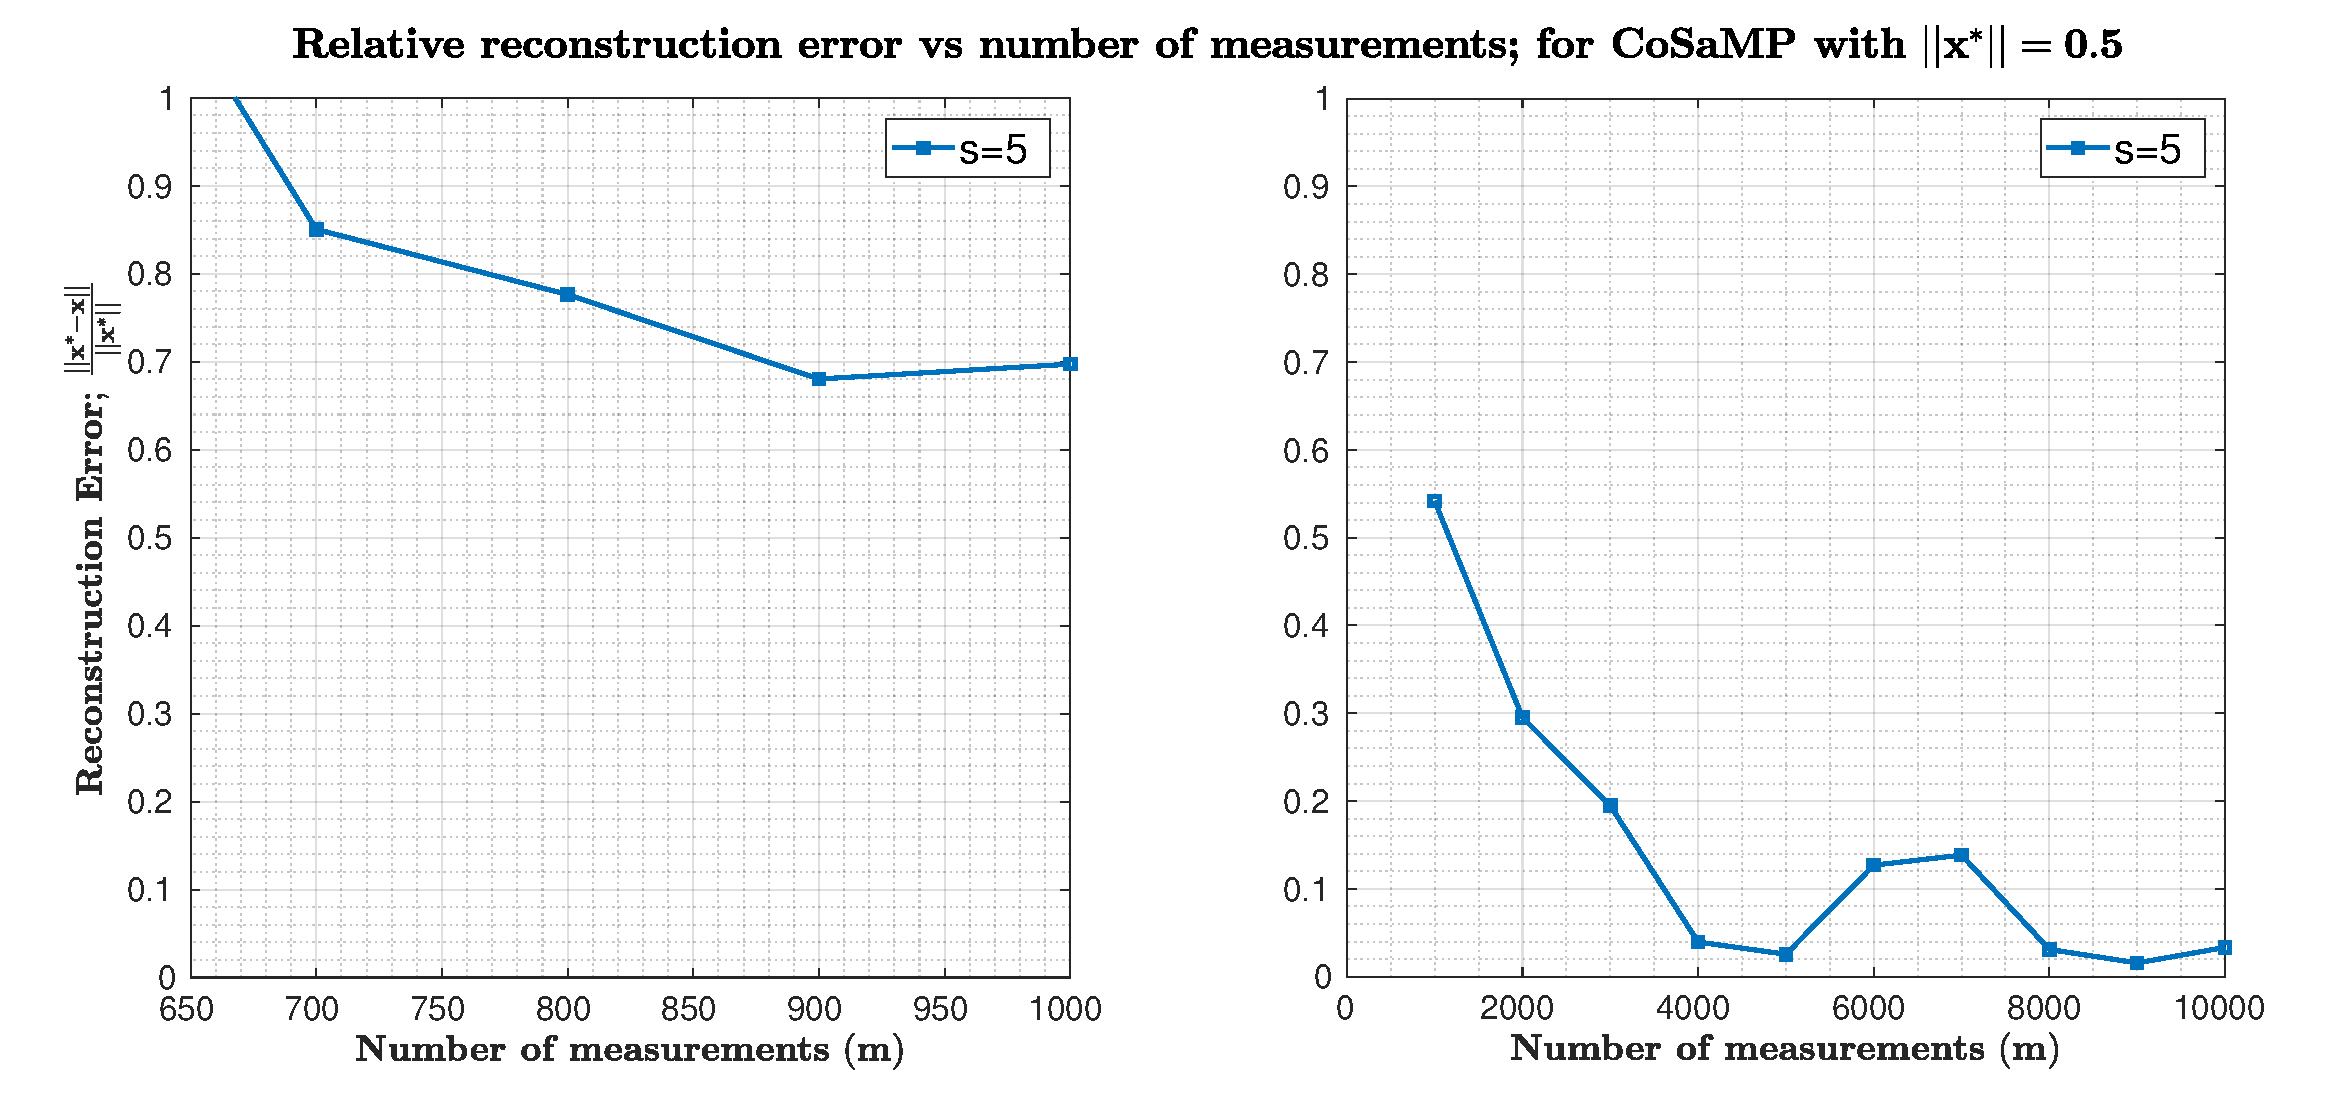
\includegraphics[width=\linewidth]{./fig/plot-1-2.pdf}
	\end{center}
	\caption{}
	\label{fig:plot-1-2}
\end{figure}
%
\begin{figure}[t]
	\begin{center}
		%\vspace{-0em}
		\includegraphics[width=\linewidth]{./fig/plot-1-3.pdf}
	\end{center}
	\caption{}
	\label{fig:plot-1-3}
\end{figure}
%
\begin{figure}[t]
	\begin{center}
		%\vspace{-0em}
		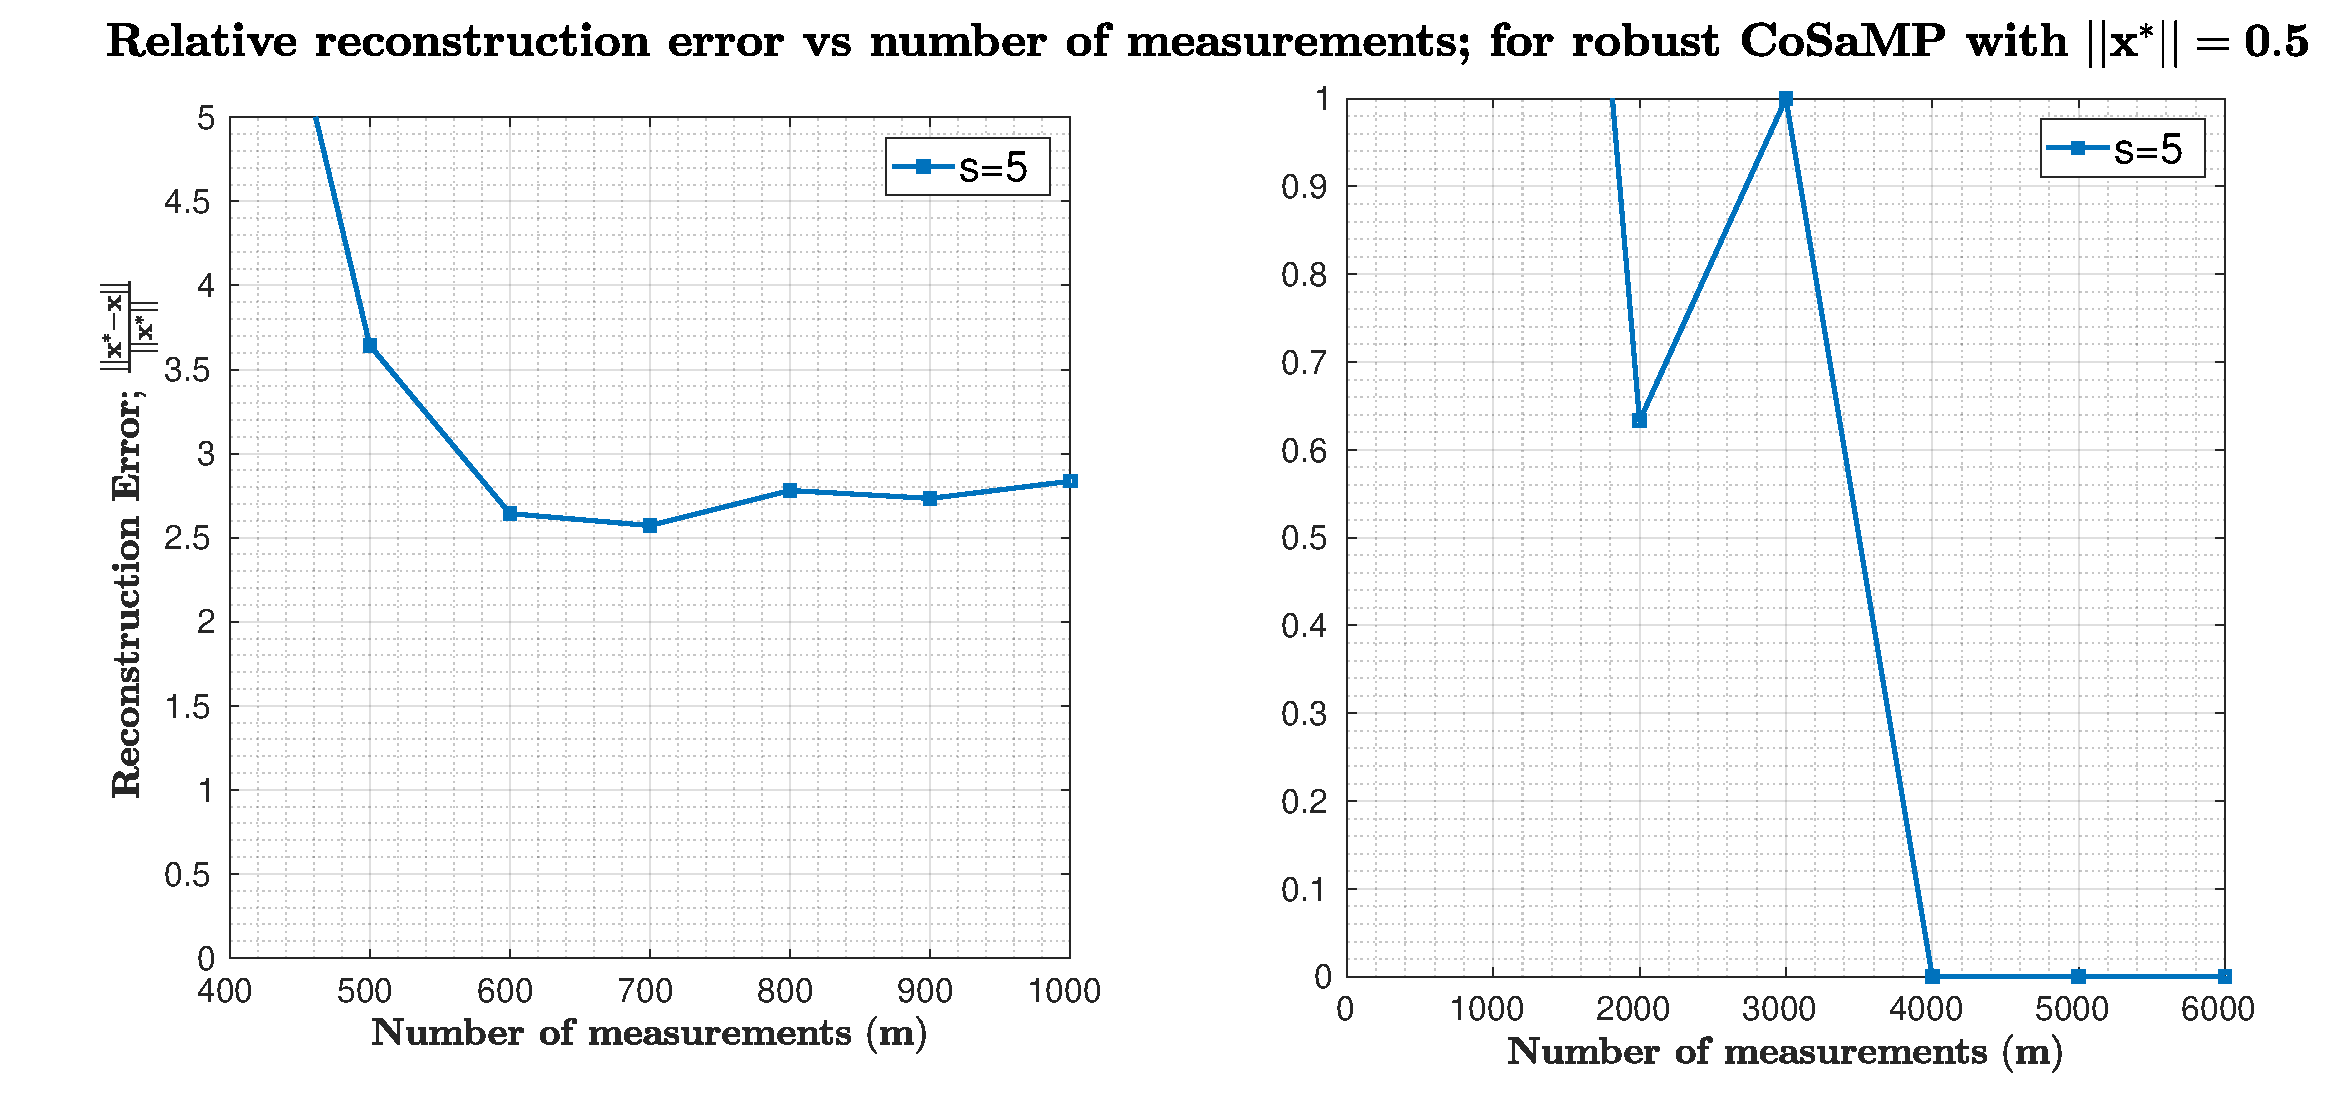
\includegraphics[width=\linewidth]{./fig/plot-1-4.pdf}
	\end{center}
	\caption{}
	\label{fig:plot-1-4}
\end{figure}






\begin{figure}[t]
	\begin{center}
		%\vspace{-0em}
		\includegraphics[width=\linewidth]{./fig/rcm_jp_r_1_s.png}
	\end{center}
	\caption{}
	\label{fig:plot-2-1}
\end{figure}


\begin{figure}[t]
	\begin{center}
		%\vspace{-0em}
		\includegraphics[width=\linewidth]{./fig/rcm_jp_r_2_s.png}
	\end{center}
	\caption{}
	\label{fig:plot-2-2}
\end{figure}


\begin{figure}[t]
	\begin{center}
		%\vspace{-0em}
		\includegraphics[width=\linewidth]{./fig/rcm_jp_r_4_s.png}
	\end{center}
	\caption{}
	\label{fig:plot-2-3}
\end{figure}




\begin{figure}[!t]
	\centering
	\subfloat[][$s=20$]{
		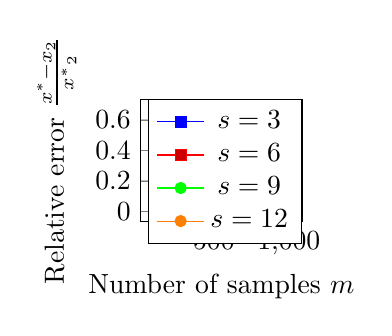
\begin{tikzpicture}
\begin{axis}
[width=0.3\textwidth,
xlabel= Number of samples $m$, 
ylabel= Relative error $\frac{\norm{\mb{x^*-x}}_2}{\norm{\mb{x^*}}_2}$,
grid style = dashed,
grid=both,
legend style=
{
at={(1,1), %for arxiv version
%at={(1.65,0.8),  %for NIPS version
anchor=top},
cells={align=center}, 
%legend columns=-1,
} 
]

\addplot[color=blue,mark=square*] plot coordinates {
	(100,     0.222952795500352)
	(200,    8.25E-05)
	(300,    6.48E-05)
	(400,    6.37E-05)
	(500,   7.91E-05)
 	(600, 6.45E-05)
	(700, 5.51E-05)
	(800, 4.77E-05)
	(900, 6.78E-05)
	(1000, 5.76E-05)
};
\addlegendentry{$s=3$};


\addplot plot coordinates {
(100,	0.391717206388554)
(200,	0.189009904901885)
(300,	8.75E-05)
(400,	6.63E-05)
(500,	7.39E-05)
(600,	6.96E-05)
(700,	5.79E-05)
(800,    6.41E-05)
(900,	8.06E-05)
(1000,	6.78E-05)
};

\addlegendentry{$s=6$};


\addplot[color=green,mark=*] plot coordinates {
(100,0.596874049564358)
(200,0.0893297570309944)
(300,0.0000961819292563893)
(400,0.0000965366166880477)
(500,0.0000950192717929039)
(600,0.0000992956375702069)
(700,0.0000835965044892149)
(800,0.0000675354618845817)
(900,0.0000811820156888768)
(1000,0.000064977150825922)
};
\addlegendentry{$s=9$};

\addplot[color=orange,mark=*] plot coordinates {
(100,0.667881390121055)
(200,0.316701449929789)
(300,0.0432277244535189)
(400,0.000108785027973407)
(500,0.0000962070190416804)
(600,0.0000899199807562489)
(700,0.000102447155819804)
(800,0.0000922462885218879)
(900,0.0000888147784526045)
(1000,0.0000753141220088111)

};
\addlegendentry{$s=12$};



%\legend{CoPRAM\\Block CoPRAM\\ThWF\\SPARTA\\}

\end{axis}
\end{tikzpicture}}
	\subfloat[][$s=30$]{
		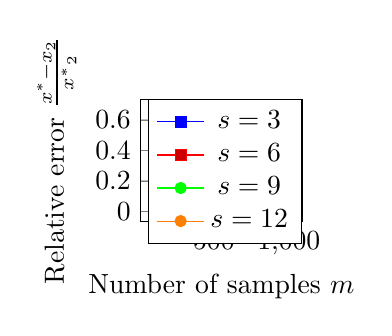
\begin{tikzpicture}
\begin{axis}
[width=0.3\textwidth,
xlabel= Number of samples $m$, 
ylabel= Relative error $\frac{\norm{\mb{x^*-x}}_2}{\norm{\mb{x^*}}_2}$,
grid style = dashed,
grid=both,
legend style=
{
at={(1,1), %for arxiv version
%at={(1.65,0.8),  %for NIPS version
anchor=top},
cells={align=center}, 
%legend columns=-1,
} 
]

\addplot[color=blue,mark=square*] plot coordinates {
	(100,     0.222952795500352)
	(200,    8.25E-05)
	(300,    6.48E-05)
	(400,    6.37E-05)
	(500,   7.91E-05)
 	(600, 6.45E-05)
	(700, 5.51E-05)
	(800, 4.77E-05)
	(900, 6.78E-05)
	(1000, 5.76E-05)
};
\addlegendentry{$s=3$};


\addplot plot coordinates {
(100,	0.391717206388554)
(200,	0.189009904901885)
(300,	8.75E-05)
(400,	6.63E-05)
(500,	7.39E-05)
(600,	6.96E-05)
(700,	5.79E-05)
(800,    6.41E-05)
(900,	8.06E-05)
(1000,	6.78E-05)
};

\addlegendentry{$s=6$};


\addplot[color=green,mark=*] plot coordinates {
(100,0.596874049564358)
(200,0.0893297570309944)
(300,0.0000961819292563893)
(400,0.0000965366166880477)
(500,0.0000950192717929039)
(600,0.0000992956375702069)
(700,0.0000835965044892149)
(800,0.0000675354618845817)
(900,0.0000811820156888768)
(1000,0.000064977150825922)
};
\addlegendentry{$s=9$};

\addplot[color=orange,mark=*] plot coordinates {
(100,0.667881390121055)
(200,0.316701449929789)
(300,0.0432277244535189)
(400,0.000108785027973407)
(500,0.0000962070190416804)
(600,0.0000899199807562489)
(700,0.000102447155819804)
(800,0.0000922462885218879)
(900,0.0000888147784526045)
(1000,0.0000753141220088111)

};
\addlegendentry{$s=12$};



%\legend{CoPRAM\\Block CoPRAM\\ThWF\\SPARTA\\}

\end{axis}
\end{tikzpicture}}
	\caption{\sl Phase transition graph for (left) $s=20$ and (right) $s=30$, for a signal of length $n=3,000$ and block length $b=5$.} \label{fig:phase_graph1}